\subsection{W-12 (SWI)}
Vzory používané během návrhu: třívrstvá architektura, Model View Controller, GoF vzory (Abstraktní továrna, Stav, Adaptér), GRASP vzory (Nízká provázanost, Vysoká soudržnost), popis spolupráce objektů (UML sekvenční diagram, UML diagram tříd).

\subsubsection*{Vícevrstvé architektury}
\begin{itemize}
  \item Monolitická = jednovrstvá. Vhodná pro prototypování
  \item Dvouvrstvá = datová + prezentační vrstva.
  \item Třívrstvá = datová, business a prezentační vrstva. (závislost prezentační->business->datová, případně může být i prezentační->datová).
\end{itemize}

\subsubsection*{Model View Controller/Presenter}
View x Controller - eventy zpracovává celé View
View x Presenter - event odchydí view, ale pošle ho do presenteru.

\subsubsection*{GoF (vytvořeno gang of four) vzory}

Dělení:
\begin{itemize}
  \item Vytváření objektů (Creational) - abstract factory, builder
  \item Vzory chování (Behavioral) - observer, strategy, state
  \item Strukturální vzory (Structural) - adapter, decorator
\end{itemize}

Jednotlivé návrhové vzory:
\begin{itemize}
  \item \textbf{Abstract factory (creational)} Abstract factory řeší problém vytváření rodiny objektů/varianty produktů. Poskytuje rozhraní pro jejich tvorbu a klient se nemusí starat o jejich variantu. Konkrétní implementace je použita konkrétní továrnou.
  \item \textbf{Builder (creational)} Jednotlivé metody builder objektu vrací Builder type objekt.
  \item \textbf{Singleton pattern (creational)} Zajišťuje, že třída má pouze jednu instanci a poskytuje globální přístup k ní. 
  \item \textbf{Adapter pattern (structural)} Adapter upravuje rozhraní objektu/třídy tak, aby bylo kompatibilní s jiným rozhraním.
  \item \textbf{Decorator pattern (structural)} Dekorátor přidává novou funkcionalitu k objektu bez změny jeho struktury. Dekorátor je podtřída třídy, kterou dekoruje.
  \item \textbf{Facade pattern (structural)} Poskytuje zjednodušené rozhraní pro složitější systém.
  \item \textbf{Chain of responsibility (behavioral)} Řetězec zpracovatelů zpracovává požadavek - každý ho buď zpracuje a nebo předá dál.
  \item \textbf{Command pattern (behavioral)} Příkaz je objekt, který encapsuluje všechny informace potřebné k provedení akce nebo události za účelem oddělení objektu, který provádí akci od objektu, který ji vyžaduje.
  \item \textbf{Iterator pattern (behavioral)} Poskytuje způsob, jak sekvenčně procházet prvky kolekce bez odhalení její vnitřní reprezentace.
  \item \textbf{Observer pattern (behavioral)} Definuje závislost mezi objekty tak, že když jeden objekt změní stav, všechny jeho závislé objekty jsou o tom informovány a automaticky aktualizovány.
  \item \textbf{Strategy pattern (behavioral)} Definuje rodinu algoritmů, zapouzdřuje je a činí je vzájemně zaměnitelnými. Strategy umožňuje algoritmu měnit chování objektu.
  \item \textbf{State pattern (behavioral)} Umožňuje objektu měnit jeho chování, když změní svůj vnitřní stav. Objekt bude vypadat, jako by změnil svou třídu. (hlavní objekt mění implementace na základě stavu)
\end{itemize}

\subsubsection*{GRASP}

Soubor devíti obecných principů návrhu objektově orientovaných systémů. Vzory GRASP se zaměřují na návrh tříd a jejich spolupráci.

\begin{itemize}
  \item \textbf{Informační expert} - přiřazení odpovědnosti třídě, která má potřebné informace pro její splnění.
  \item \textbf{Nízká provázanost} - minimalizace závislostí mezi třídami. Třídy by měly být co nejvíce nezávislé.
  \item \textbf{Vysoká soudržnost} - třída by měla mít co nejvíce souvisejících odpovědností, třída by měla mít jasný úkol.
\end{itemize}

\subsubsection*{Sekvenční diagram}

%screenshot_2025-05-14_09-50-25.png
\begin{figure}[H]
  \centering
  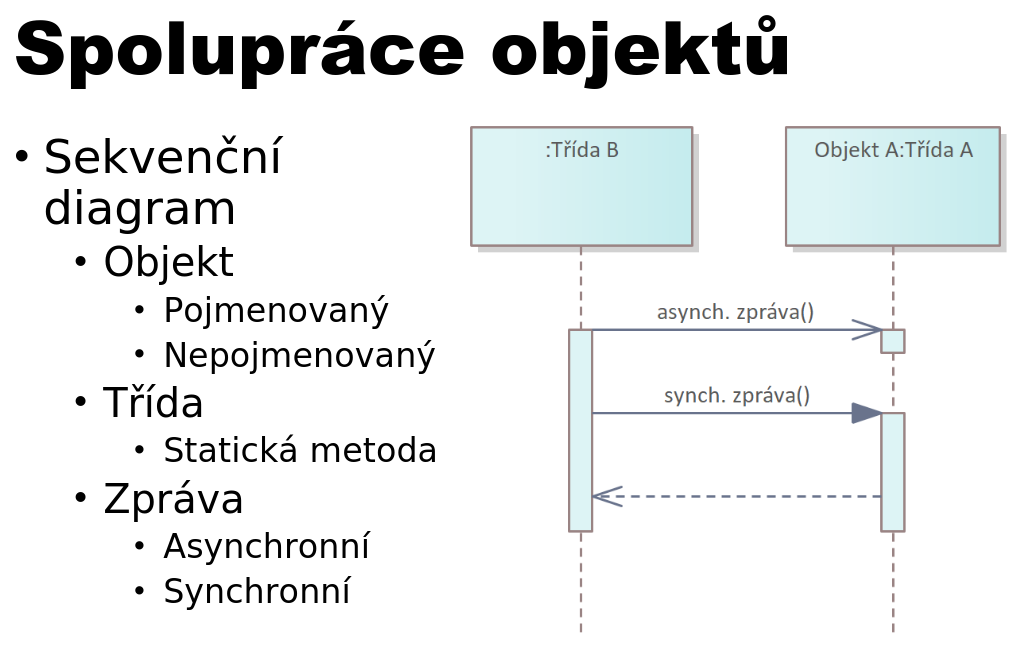
\includegraphics[width=0.8\textwidth]{img/screenshot_2025-05-14_09-50-25.png}
  \caption{Sekvenční diagram}
  \label{fig:sekv_diagram}
\end{figure}

